\documentclass{article}
\author{Grunda}
% Підключення додаткових пакетів
\usepackage[utf8]{inputenc} 
\usepackage[ukrainian]{babel}  
\usepackage{amsmath}  
\usepackage{graphicx} 
\usepackage{amsfonts} 
\usepackage{geometry}  
\usepackage{color}
\usepackage{listings}   % для відображення коду
\usepackage{color}      % для кольорів у коді
\usepackage{caption}    % для підписів до фігур/таблиць
\usepackage{hyperref}   % для гіперпосилань
\usepackage{tikz}
\usetikzlibrary{arrows.meta}
\geometry{left=2.5cm, right=2.5cm, top=2.5cm, bottom=2.5cm}

% Титульна сторінка
\title{Звіт до лабораторної роботи}
\author{Ярослав Грунда \\ Фі-21, ФТІ КПІ}
\date{\today}

\begin{document}

\maketitle

\tableofcontents  % Зміст
\newpage

\section{Мета роботи}
Опанувати способи реалізації представлення різних типів графів (неорієнтовані, орієнтовані, зважені) та їх ефективної реалізації.

\section{Опис класів}
\subsection{Структура коду}
\begin{center} 
\begin{tikzpicture}[
    node distance=4cm,
    every node/.style={draw, rectangle, rounded corners, align=center, minimum width=3cm}
    ]

    % Вузли
    \node (baseGraph) {baseGraph};
    \node (graph) [left of=baseGraph] {Graph};
    \node (weightedGraph) [right of=baseGraph] {weightedGraph};
    \node (orientedGraph) [below of=graph] {orientedGraph};
    \node (orientedWeightedGraph) [below of=weightedGraph] {orientedWeightedGraph};
    \node (randomOrientedGraph) [below of=orientedGraph] {randomOrientedGraph};
    \node (randomOrientedWeightedGraph) [below of=orientedWeightedGraph] {randomOrientedWeightedGraph};

    % Стрілки
    \draw[-{Stealth[scale=1.5]}] (baseGraph) -- (graph);
    \draw[-{Stealth[scale=1.5]}] (baseGraph) -- (weightedGraph);
    \draw[-{Stealth[scale=1.5]}] (baseGraph) -- (orientedGraph);
    \draw[-{Stealth[scale=1.5]}] (baseGraph) -- (orientedWeightedGraph);
    \draw[-{Stealth[scale=1.5]}] (orientedGraph) -- (randomOrientedGraph);
    \draw[-{Stealth[scale=1.5]}] (orientedWeightedGraph) -- (randomOrientedWeightedGraph);

\end{tikzpicture}
\end{center}
\subsection{Клас \texttt{baseGraph}}
Цей клас є базовим для всіх графів. Він ініціалізує порожній граф з заданою кількістю вершин і містить методи для додавання та видалення вершин, а також для перетворення графа між списком і матрицею суміжності.
\begin{itemize}
    \item \texttt{def \_\_init\_\_(self, n):} - Ініціалізація порожнього графа з n вершинами.
    \item \texttt{def add\_vertex(self):} - Додає нову вершину до графа.
    \item \texttt{def del\_vertex(self, v):} - Видаляє вершину v і всі пов'язані з нею ребра.
    \item \texttt{def to\_adjacency\_matrix(self):} - Перетворює граф зі списку суміжності у матрицю суміжності.
    \item \texttt{def to\_adjacency\_list(self, matrix, weighted=False):} - Перетворює граф з матриці суміжності у список суміжності.
    \item \texttt{def show(self):} - Виводить граф у вигляді списку суміжності.
    \item \texttt{def show\_matrix(self):} - Виводить граф у вигляді матриці суміжності.
    \item \texttt{def makeNonOriented(self):} - Робить граф неорієнтованим.
\end{itemize}


\textbf{Швидкості функцій:}
\begin{itemize}
    \item \texttt{add\_vertex()}: $O(1)$
    \item \texttt{del\_vertex(v)}: $O(V + E)$, де $V$ — кількість вершин, $E$ — кількість ребер.
    \item \texttt{to\_adjacency\_matrix()}: $O(V^2)$
    \item \texttt{to\_adjacency\_list(matrix, weighted)}: $O(V^2)$
    \item \texttt{show()}: $O(V)$
    \item \texttt{show\_matrix()}: $O(V^2)$
\end{itemize}

\subsection{Клас \texttt{Graph}}
Цей клас реалізує неорієнтований граф. Він має методи для додавання та видалення ребер.

\begin{itemize}
    \item \texttt{def add\_edge(self, u, v):} - Додає ребро між вершинами u і v.
    \item \texttt{def del\_edge(self, u, v):} - Видаляє ребро між вершинами u і v.
\end{itemize}


\textbf{Швидкості функцій:}
\begin{itemize}
    \item \texttt{add\_edge(u, v)}: $O(V)$
    \item \texttt{del\_edge(u, v)}: $O(V)$
\end{itemize}

\subsection{Клас \texttt{weightedGraph}}
Цей клас реалізує зважений неорієнтований граф.
\begin{itemize}
    \item \texttt{def add\_edge(self, u, v, w):} - Додає зважене ребро між вершинами u і v з вагою w.
    \item \texttt{def del\_edge(self, u, v):} - Видаляє зважене ребро між вершинами u і v.
\end{itemize}

    
\textbf{Швидкості функцій:}
\begin{itemize}
    \item \texttt{add\_edge(u, v, w)}: $O(V)$
    \item \texttt{del\_edge(u, v)}: $O(V)$
\end{itemize}

\subsection{Клас \texttt{orientedGraph}}
Цей клас реалізує орієнтований граф.

\begin{itemize}
    \item \textbf{class orientedGraph(baseGraph):}
    \begin{itemize}
        \item \texttt{def add\_edge(self, u, v):} - Додає орієнтоване ребро між вершинами u і v.
        \item \texttt{def del\_edge(self, u, v):} - Видаляє орієнтоване ребро між вершинами u і v.
    \end{itemize}
\end{itemize}

\textbf{Швидкості функцій:}
\begin{itemize}
    \item \texttt{add\_edge(u, v)}: $O(V)$
    \item \texttt{del\_edge(u, v)}: $O(V)$
\end{itemize}

\subsection{Клас \texttt{orientedWeightedGraph}}
Цей клас реалізує зважений орієнтований граф.

\begin{itemize}
    \item \texttt{def add\_edge(self, u, v, w):} - Додає орієнтоване зважене ребро (u --w--> v) до графа.
    \item \texttt{def del\_edge(self, u, v):} - Видаляє орієнтоване зважене ребро (u --w--> v) з графа.
\end{itemize}


\textbf{Швидкості функцій:}
\begin{itemize}
    \item \texttt{add\_edge(u, v, w)}: $O(V)$
    \item \texttt{del\_edge(u, v)}: $O(V)$
\end{itemize}

\subsection{Клас \texttt{randomOrientedGraph}}
Цей клас реалізує випадковий орієнтований граф у моделі Ердеша-Шеньї.
\begin{itemize}
    \item \texttt{def \_\_init\_\_(self, n, p):} - Ініціалізує випадковий орієнтований граф з n вершинами і ймовірністю p для створення ребра.
    \item \texttt{def generate\_random\_graph(self, p):} - Генерує випадковий орієнтований граф за імовірністю p для кожної пари вершин.
\end{itemize}

\textbf{Швидкості функцій:}
\begin{itemize}
    \item \texttt{generate\_random\_graph(p)}: $O(V^2)$
\end{itemize}

\subsection{Клас \texttt{randomOrientedWeightedGraph}}
Цей клас реалізує випадковий орієнтований граф у моделі Ердеша-Шеньї.
\begin{itemize}
    \item \texttt{def \_\_init\_\_(self, n, p, min\_weight=1, max\_weight=10):} - Ініціалізує випадковий зважений граф з n вершинами, ймовірністю p для створення ребра, і вагою між min\_weight та max\_weight.
    \item \texttt{def generate\_random\_graph(self, p, min\_weight, max\_weight):} - Генерує випадковий зважений граф за ймовірністю p для кожної пари вершин з випадковою вагою.
\end{itemize}

\textbf{Швидкості функцій:}
\begin{itemize}
    \item \texttt{generate\_random\_graph(p, min\_weight, max\_weight)}: $O(V^2)$
\end{itemize}
\section{Тестування швидкості}
\subsection{Результати ініціювання графа без ребер}

\begin{figure}[h!]
\centering
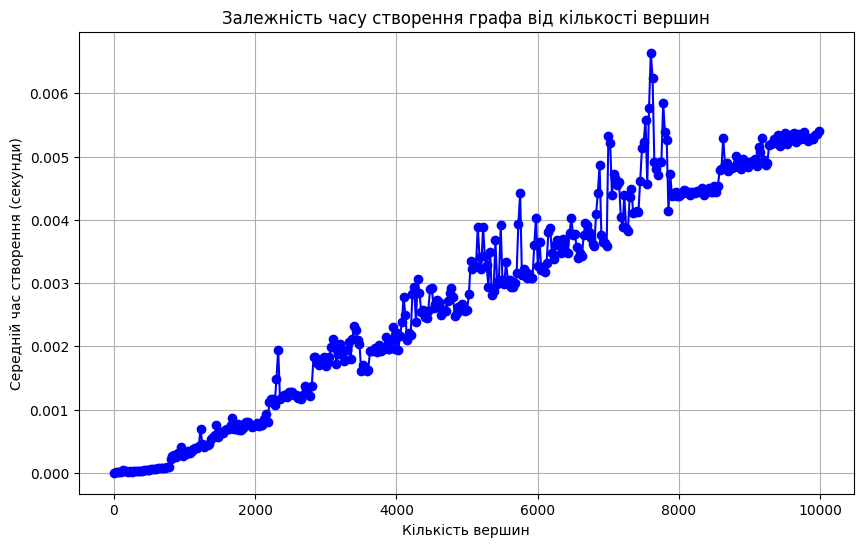
\includegraphics[width=0.8\textwidth]{img/init.png}
\caption{Бачимо лінійну складність, що пояснюється тим що створення кожної вершини і порожнього списку сусідів має постійну складність $O(1)$, оскільки таких ітерацій n, загальна складність цієї операції — $O(deg V)$.}
\label{fig:init}
\end{figure}

\subsection{Результати додавання та видалення (видалення для орієнтованого графа) вершин}

\begin{figure}[h!]
\centering
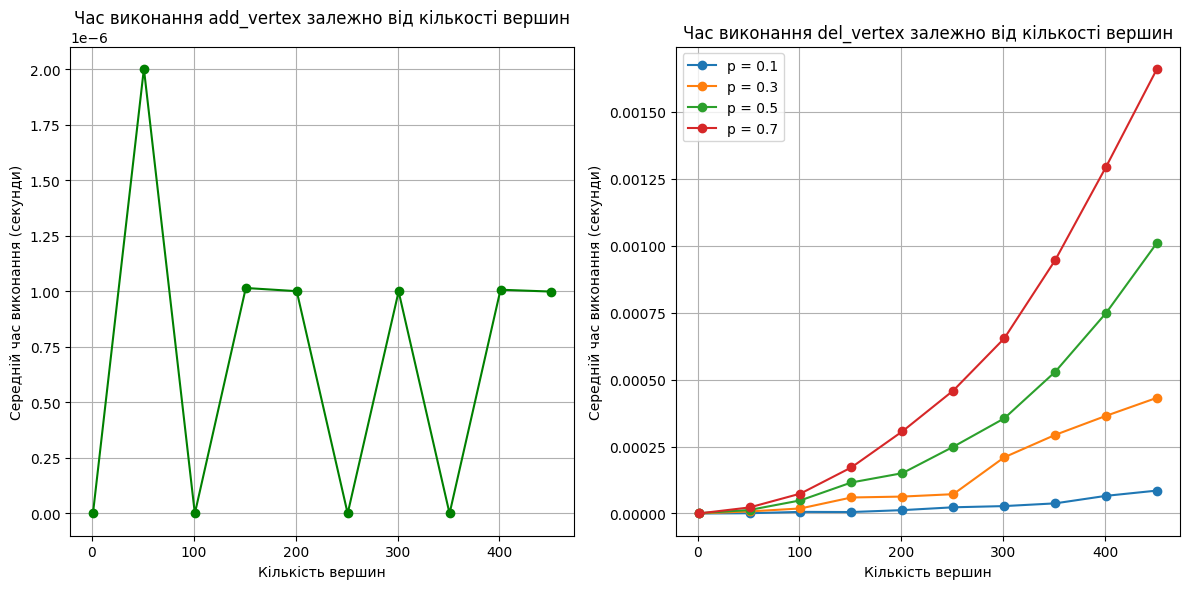
\includegraphics[width=0.8\textwidth]{img/vertex.png}
\caption{Для додавання очевидно складність $O(1)$, оскільки це просто створення нового пустого списку. Для видалення бачимо ріст при збільшенні кількості вершин і залежність від щільності графа, тому $O(deg V)$}
\label{fig:add, del vertexes}
\end{figure}

\subsection{Результати додавання та видалення ребра (для орієнтованого графа)}
\begin{figure}[h!]
\centering
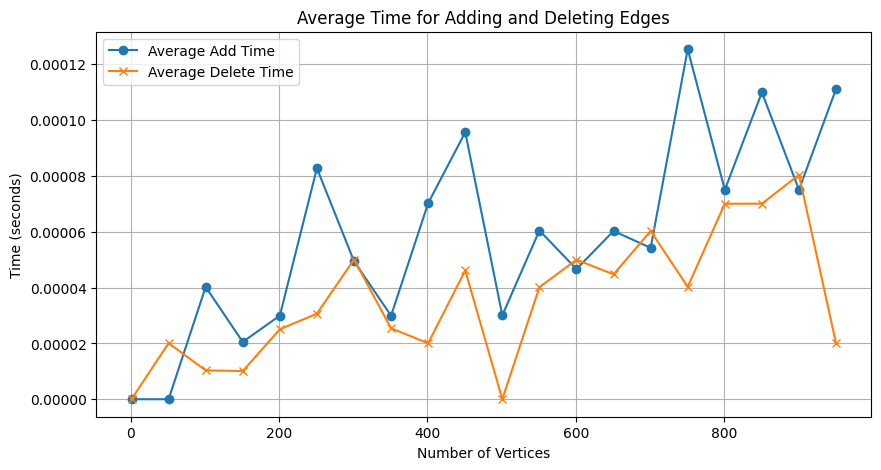
\includegraphics[width=0.8\textwidth]{img/edges2.png}
\caption{Бачимо ріст при збільшенні вершин, але оскільки додавання і видалення залежать від щільності графа, тобто $O(deg_V)$}, бо потрібно перевірити чи існує ребро перед тим як додати чи прибрати його, тому значення доволі не лінійні.
\label{fig:add, del edges}
\end{figure}

\newpage

\subsection{Результати генерування випадкових орієнтованих графів}
\begin{figure}[h!]
\centering
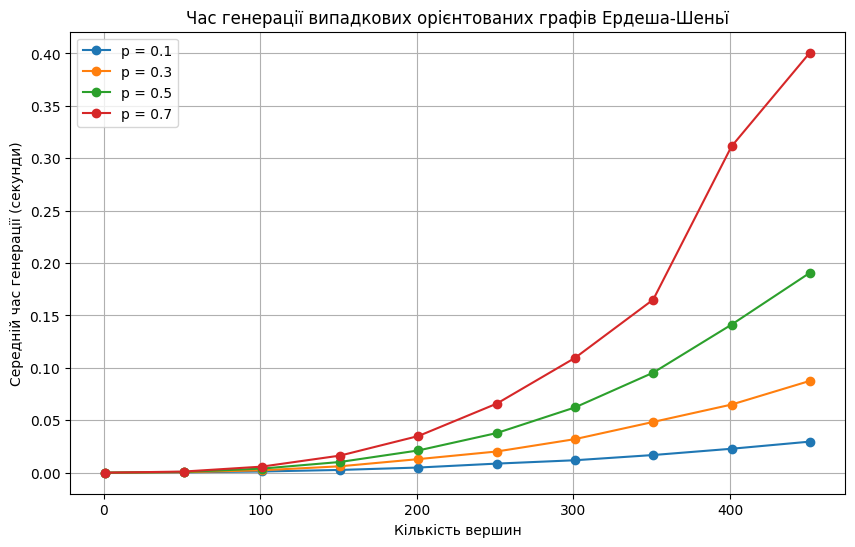
\includegraphics[width=0.8\textwidth]{img/randomgraphs.png}
\caption{Бачимо для щільного графа $O(V^2)$, для розрідженого схоже на лінійну складність $O(V)$}
\label{fig:random graphs}
\end{figure}
    
\section{Висновки}

У процесі виконання лабораторної роботи ми дослідили різні способи представлення графів, включаючи неорієнтовані, орієнтовані та зважені графи. Реалізація класів дозволила зрозуміти структуру та ефективність різних операцій, таких як додавання та видалення вершин і ребер.

Аналіз швидкостей функцій показав, що:
\begin{itemize}
    \item Додавання нових вершин має постійну складність \(O(1)\).
    \item Видалення вершин і ребер залежить від кількості сусідів, що веде до складності \(O(deg \, V)\).
    \item Генерація випадкових графів демонструє квадратичну складність \(O(V^2)\) для щільних графів, тоді як для розріджених графів складність наближається до лінійної.
\end{itemize}

Для більш детальної інформації, будь ласка, відвідайте наступний ресурс:
\href{https://github.com/gre1wy/AppliedAlgorithms/tree/main/lab1}{Перейти до репозиторію}.

\end{document}
